\documentclass{IEEEtran}
\usepackage{cite}
\usepackage{amsmath,amssymb,amsfonts}
\usepackage{graphicx}
\usepackage{textcomp}
\usepackage{xcolor}
\usepackage{booktabs}
\usepackage{multirow}
\usepackage{url}
\usepackage{hyperref}
\usepackage{stfloats}
\usepackage{tipa}
\graphicspath{{./}}

\def\BibTeX{{\rm B\kern-.05em{\sc i\kern-.025em b}\kern-.08em
    T\kern-.1667em\lower.7ex\hbox{E}\kern-.125emX}}

\markboth{STUDENT SCIENTIFIC RESEARCH COMMUNICATION, VOLUME I, 2026}
{Nguyen \MakeLowercase{\textit{et al.}}: IELTS Master English AI}
\begin{document}

\title{IELTS Master English AI: An AI-Powered IELTS Preparation Platform with LLM-Based Assessment, Multi-Metric Pronunciation Scoring, and Adaptive Spaced Repetition}

\author{Nguyen Thi Hoang Khanh, Pham Duc Tai, and Lai Thanh Si
\thanks{N. T. H. Khanh is with the Faculty of Information Technology, Industrial University of Ho Chi Minh City, Vietnam (e-mail: nguyenthihoangkhanh@iuh.edu.vn).}
\thanks{P. D. Tai is with the Faculty of Information Technology, Industrial University of Ho Chi Minh City, Vietnam (e-mail: tylerpham102703@gmail.com).}
\thanks{L. T. Si is with the Faculty of Information Technology, Industrial University of Ho Chi Minh City, Vietnam (e-mail: lathanhsi100804@gmail.com).}}

\maketitle

% ============================================================
% ABSTRACT
% ============================================================

\begin{abstract}
Automated assessment of subjective English language skills remains an open challenge in computer-assisted language learning. This paper presents a comprehensive preparation platform for the International English Language Testing System (IELTS) built on an event-driven hybrid architecture that separates artificial intelligence inference from core application logic via asynchronous message brokering. The platform implements three principal techniques: large language model based writing and speaking grading with structured rubric output aligned to official IELTS band descriptors, multimodal speaking assessment combining local speech-to-text transcription with direct audio analysis for pronunciation and fluency evaluation, and adaptive spaced repetition vocabulary scheduling with bounded interval growth. Preliminary validation on 30 human-scored IELTS essays demonstrates strong inter-rater agreement between the automated grader and human examiners, achieving a Pearson correlation of 0.97, a quadratic-weighted Cohen's kappa of 0.96, and 96.7\% of predicted scores falling within half a band of the human reference. A dedicated multi-metric pronunciation scoring pipeline achieves strong error-severity discrimination with a Spearman rank correlation of $-$0.957. Stochastic simulation further verifies that the spaced repetition implementation produces bounded, adaptive review intervals that correctly differentiate across learner proficiency levels.
\end{abstract}

\begin{IEEEkeywords}
IELTS preparation, automated essay scoring, multimodal speech assessment, spaced repetition, event-driven architecture, large language models
\end{IEEEkeywords}

% ============================================================
\section{Introduction}
% ============================================================

The International English Language Testing System (IELTS) is recognized by over 11{,}000 organizations across 140 countries, making it the world's most widely accepted English proficiency test for higher education admissions and skilled migration~\cite{ielts_stats}. With over 3.5 million tests administered annually, there is significant demand for accessible, technology-driven preparation tools that can provide formative feedback on all four language skills---Listening, Reading, Writing, and Speaking. While objective skills (Listening, Reading) can be scored algorithmically through answer-key matching, the subjective skills (Writing, Speaking) require nuanced evaluation against multi-dimensional rubrics, a task that has historically required trained human examiners.

Recent advances in large language models (LLMs) have opened new possibilities for automated subjective assessment. However, a survey of existing IELTS preparation platforms reveals three persistent gaps:

\textbf{Gap~1: No validated LLM-based IELTS grading.} Although automated essay scoring (AES) is a well-established research field~\cite{erater,aes_handbook}, no commercially available platform provides LLM-based grading for both Writing and Speaking that has been empirically validated against human examiner scores with per-criterion statistical analysis. Existing platforms either omit subjective-skill feedback entirely or rely on unvalidated LLM output without reporting agreement metrics.

\textbf{Gap~2: Cloud-dependent speech processing.} Pronunciation and fluency assessment in current platforms typically requires expensive cloud APIs such as Google Cloud Speech or Azure Speech Services. No existing system combines local speech-to-text processing with multimodal LLM grading that evaluates pronunciation and fluency directly from audio signals rather than text transcripts alone.

\textbf{Gap~3: No adaptive vocabulary system for IELTS.} While spaced repetition algorithms such as SM-2~\cite{sm2} and FSRS~\cite{fsrs} have been extensively studied in the memory science literature, they are rarely integrated into IELTS-specific vocabulary acquisition workflows that align review content with test preparation objectives.

This paper presents IELTS Master English AI, a full-stack educational platform that addresses these gaps through an event-driven hybrid architecture combining a NestJS modular monolith with a dedicated Python FastAPI microservice for AI inference. The system employs Gemini 2.5 Flash~\cite{gemini} for structured writing grading and multimodal speaking assessment, Faster-Whisper~\cite{faster_whisper} for local speech-to-text processing, and the FSRS algorithm~\cite{fsrs} for adaptive vocabulary scheduling. Preliminary validation on a stratified sample of 30 human-scored IELTS essays demonstrates strong inter-rater agreement, supporting the viability of LLM-based grading as a formative assessment tool.

The remainder of this paper is organized as follows. Section~\ref{sec:background} surveys related work in automated assessment and spaced repetition. Section~\ref{sec:system} details the system architecture and implementation. Section~\ref{sec:evaluation} presents the experimental evaluation. Section~\ref{sec:conclusion} concludes with limitations and future directions.

% ============================================================
\section{Background and Related Work}
\label{sec:background}
% ============================================================

\subsection{Automated Assessment in Language Learning}

Automated Essay Scoring (AES) has a decades-long research history. Early systems such as Page's Project Essay Grade (1966) relied on surface-level textual features. The Educational Testing Service's e-rater~\cite{erater} advanced the field by combining over 100 hand-crafted features---including discourse structure, vocabulary sophistication, and grammatical accuracy---to predict holistic essay scores. The Automated Student Assessment Prize (ASAP) Kaggle competition~\cite{asap} subsequently demonstrated that neural approaches could match or exceed feature-engineered systems on standardized essay prompts.

More recently, large language models have emerged as a new paradigm for automated assessment. Mizumoto and Eguchi~\cite{llm_aes} demonstrated that GPT-based models can achieve inter-rater reliability comparable to human examiners on standardized writing tasks when provided with structured rubric prompts and constrained output formats. This finding suggests that LLMs, when properly prompted, can serve as reliable automated graders for subjective writing tasks.

For speaking assessment, Computer-Assisted Pronunciation Training (CAPT) systems have traditionally relied on Goodness of Pronunciation (GOP) scoring~\cite{gop_scoring}, which compares forced-aligned phoneme likelihoods against native speaker distributions. Commercial platforms such as ELSA Speak provide phoneme-level feedback but require cloud API access and proprietary models. A newer approach, enabled by multimodal LLMs such as Gemini~\cite{gemini}, involves sending raw audio directly to the model for holistic evaluation---eliminating the need for separate pronunciation assessment pipelines entirely.

This system adopts LLM-based assessment using Gemini 2.5 Flash as a unified grading backbone for both Writing and Speaking. The key gap addressed is that no prior system has validated LLM-based IELTS grading against human examiner band scores with per-criterion statistical analysis across Task Achievement, Coherence and Cohesion, Lexical Resource, and Grammatical Range and Accuracy.

\subsection{Spaced Repetition for Vocabulary Acquisition}

Spaced repetition exploits the spacing effect---first documented by Ebbinghaus in 1885~\cite{ebbinghaus}---to optimize long-term memory retention by scheduling reviews at increasing intervals. The Leitner system (1972) introduced a simple box-based scheduling mechanism, while the SM-2 algorithm~\cite{sm2}, developed by Wozniak in 1990, formalized the approach with a quality-rating-driven ease factor that adapts review intervals over time. SM-2 remains the default scheduler in Anki and has been widely adopted in educational technology.

However, SM-2 exhibits two well-documented limitations: unbounded interval growth (where high-performing cards can reach intervals exceeding 200 years) and a fixed-formula ease factor that does not adapt to individual learner forgetting curves. The Free Spaced Repetition Scheduler (FSRS)~\cite{fsrs}, proposed by Ye in 2022, addresses these limitations with a Difficulty--Stability--Retrievability (DSR) model trained on over 700 million review records from Anki users. FSRS models memory retrievability as:
\begin{equation}
R(t) = \left(1 + \frac{t}{9 \cdot S}\right)^{-1}
\label{eq:retrievability}
\end{equation}
where $t$ is elapsed days since the last review and $S$ is the card's stability parameter. The next review is scheduled when $R$ drops below the configured retention threshold. Comparative studies show FSRS outperforms SM-2 in retention prediction accuracy across diverse user populations.

This system integrates the \texttt{ts-fsrs} TypeScript library with parameters \texttt{request\_retention=0.9} and \texttt{maximum\_interval=365}, ensuring intervals are both adaptive to individual performance and bounded to prevent pathological scheduling.

\subsection{Comparison with Existing Platforms}

Table~\ref{tab:comparison} compares the proposed system with four representative platforms across key technical capabilities. The comparison includes features where the proposed system is weaker (gamification, offline mode, community) to provide an honest assessment of the competitive landscape.

\begin{table*}[!t]
\caption{Feature Comparison of IELTS Preparation Platforms}
\label{tab:comparison}
\centering
\begin{tabular}{lccccc}
\toprule
\textbf{Feature} & \textbf{This System} & \textbf{Duolingo} & \textbf{ELSA Speak} & \textbf{British Council} & \textbf{Magoosh} \\
\midrule
IELTS 4-skill mock exams      & \checkmark           & --          & --              & Limited          & \checkmark \\
AI Writing grading (validated) & \checkmark           & --          & --              & --               & -- \\
Multimodal Speaking grading    & \checkmark           & --          & Phoneme-level   & --               & -- \\
Local STT (no cloud API)       & \checkmark           & --          & --              & --               & -- \\
Adaptive spaced repetition     & FSRS                 & --          & --              & --               & -- \\
Personalized learning pathway  & \checkmark           & \checkmark  & --              & --               & -- \\
Gamification                   & --                   & \checkmark  & \checkmark      & --               & -- \\
Offline mode                   & --                   & \checkmark  & \checkmark      & --               & -- \\
Community features             & --                   & \checkmark  & --              & --               & -- \\
\bottomrule
\end{tabular}
\end{table*}

The principal differentiators of this system are: (1)~empirically validated LLM-based grading for subjective IELTS skills, (2)~multimodal speaking assessment that evaluates pronunciation and fluency directly from audio rather than text transcripts alone, and (3)~FSRS-based vocabulary scheduling integrated with IELTS-specific content and a personalized learning pathway.

% ============================================================
\section{System Design and Implementation}
\label{sec:system}
% ============================================================

\subsection{Architecture Overview}

The platform follows a three-layer event-driven hybrid architecture, illustrated in Fig.~\ref{fig:architecture}. The \textbf{Client layer} comprises a Next.js~14 web application and a React Native/Expo mobile client, both communicating via REST APIs. The \textbf{Application layer} consists of two backend services: a NestJS modular monolith handling business logic, authentication, exam management, and data persistence; and a FastAPI microservice dedicated to AI inference workloads (writing grading, speaking grading, pronunciation analysis). RabbitMQ serves as the message broker between these services for asynchronous tasks. The \textbf{Data layer} includes PostgreSQL~16 for relational storage, Redis~7 for caching and session management, and MinIO for audio file storage.

The hybrid monolith-plus-microservice pattern was chosen because AI workloads require the Python ecosystem (PyTorch, faster-whisper, Google Generative AI SDK) and exhibit fundamentally different resource profiles---inference latency of 3--25 seconds versus sub-100ms for standard API operations. Isolating the AI service enables independent scaling, separate dependency management, and zero-downtime model updates.

\begin{figure}[htbp]
\centerline{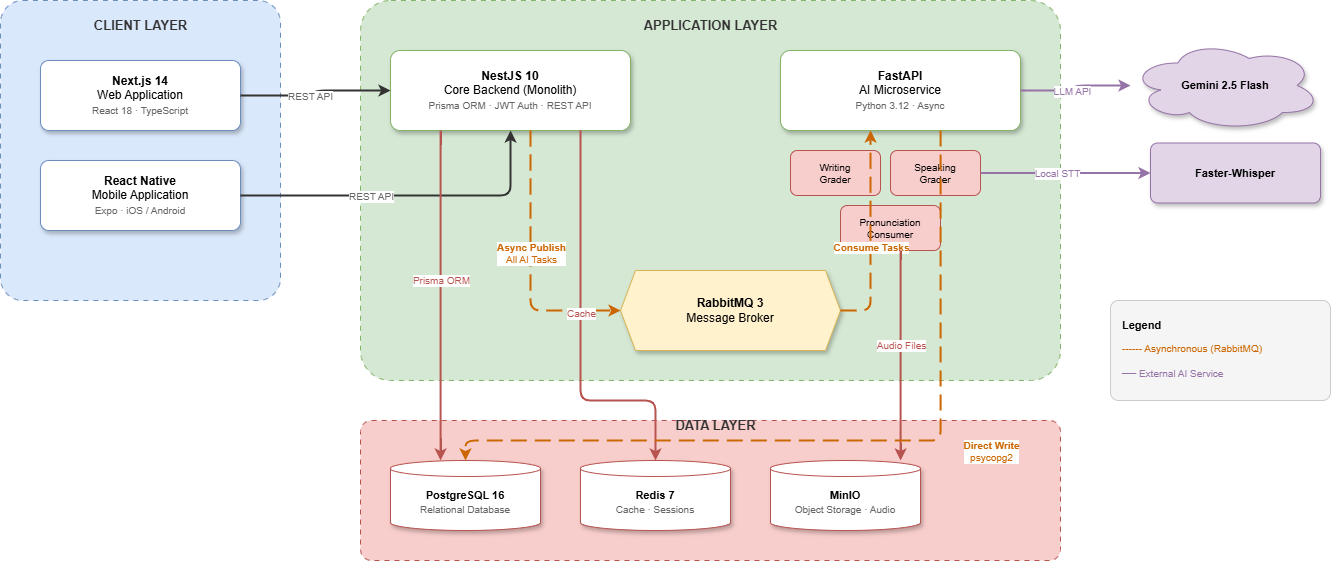
\includegraphics[width=\columnwidth,keepaspectratio]{fig1.png}}
\caption{System architecture overview showing the three-layer event-driven hybrid design. The NestJS core backend handles business logic and data persistence, while the FastAPI AI microservice processes writing grading, speaking grading, and pronunciation analysis. RabbitMQ decouples asynchronous AI tasks from the synchronous API.}
\label{fig:architecture}
\end{figure}

\subsection{Event-Driven AI Processing Pipeline}

To ensure high availability and prevent long-running inference (which can take 3--25 seconds) from blocking the main API thread pool, the system employs a fully asynchronous, event-driven pipeline for all AI workloads (Writing, Speaking, and Pronunciation grading). 

When a user submits an essay or speaking test, the NestJS core backend immediately returns a \texttt{202 Accepted} status and publishes a task payload to the \texttt{exam-grading-queue} in RabbitMQ. A dedicated pool of Python consumers running in the FastAPI microservice listens to this queue. For Writing tasks, the consumer structures the prompt and invokes the Gemini 2.5 Flash API. For Speaking and Pronunciation tasks, the consumer first downloads the audio from MinIO, transcribes it via Faster-Whisper, and then performs either LLM grading or IPA phoneme comparison. 

Once grading is complete, the Python consumer writes the results directly to the PostgreSQL \texttt{results} table via \texttt{psycopg2} and updates the exam session status to \texttt{GRADED}. The React client maintains a non-blocking UI state and polls the backend for completion. This fire-and-forget message broker pattern decouples the computationally expensive AI inference from the user-facing web server, allowing for independent scaling and robust fault tolerance (e.g., using Dead Letter Exchanges for failed inferences).

\subsection{Writing Assessment Pipeline}

The writing grader uses Gemini 2.5 Flash with \texttt{response\_mime\_type="application/json"} to guarantee well-formed structured output. A carefully engineered system prompt instructs the model to evaluate each essay against the four official IELTS Writing band descriptors:

\begin{enumerate}
\item \textbf{Task Achievement} (TA): How well the candidate addresses all parts of the task
\item \textbf{Coherence and Cohesion} (CC): Logical organization and use of cohesive devices
\item \textbf{Lexical Resource} (LR): Range and accuracy of vocabulary
\item \textbf{Grammatical Range and Accuracy} (GRA): Variety and correctness of grammatical structures
\end{enumerate}

For each criterion, the model outputs a band score (1.0--9.0 in 0.5 increments), lists of specific strengths, weaknesses, actionable improvement suggestions, and up to 10 annotated language mistakes with corrections and explanations.

To prevent arithmetic errors from the LLM, band scores are recalculated server-side:
\begin{equation}
\text{Overall} = \text{round}_{0.5}\negmedspace\left(\frac{B_{\text{Task1}} + B_{\text{Task2}} \times 2}{3}\right)
\label{eq:overall}
\end{equation}
where $B_{\text{Task1}}$ and $B_{\text{Task2}}$ are the mean of the four criterion scores for each task, rounded to the nearest 0.5. If JSON parsing fails, the system falls back to a zeroed-score response with a diagnostic error message, ensuring the pipeline never fails silently.

\subsection{Multimodal Speaking Assessment}

The speaking grader implements a four-stage multimodal pipeline that provides Gemini with both audio and text evidence for comprehensive evaluation:

\textbf{Stage~1 --- Audio decoding.} Candidate recordings, submitted as Base64-encoded WebM or URL references, are decoded into temporary audio files.

\textbf{Stage~2 --- Local transcription.} Each audio file is processed by Faster-Whisper~\cite{faster_whisper,whisper_paper} running locally with beam search ($\text{beam\_size}=5$), Voice Activity Detection (VAD) filtering, and \texttt{word\_timestamps=True}. This produces both a full transcript and per-word probability scores, enabling fine-grained confidence analysis without cloud API dependency.

\textbf{Stage~3 --- Multimodal prompt construction.} The system constructs a composite content array containing: (a)~raw audio bytes submitted via \texttt{types.Part.from\_bytes()} for direct audio analysis by Gemini, and (b)~a formatted text transcript annotated with per-word Whisper confidence scores. Words with confidence below 0.7 are explicitly flagged (e.g., ``\textit{[STT Confidence: 0.62 | Low confidence words: particularly, consciousness]}''), directing Gemini's attention to potential pronunciation difficulties.

\textbf{Stage~4 --- LLM evaluation.} Gemini 2.5 Flash evaluates the combined audio-plus-text input against four IELTS Speaking criteria: Fluency and Coherence, Lexical Resource, Grammatical Range and Accuracy, and Pronunciation. The system prompt explicitly instructs the model to base Pronunciation and Fluency assessments on the \emph{audio signal}, not the text transcript, since text cannot capture hesitation, intonation, or phoneme-level errors.

This multimodal architecture is a key differentiator: by submitting audio directly alongside confidence-annotated transcripts, the system enables evaluation of suprasegmental features (stress, rhythm, intonation) that are invisible in text-only approaches.

\subsection{Pronunciation Practice Scoring}

Distinct from the holistic Speaking exam grader described above, the platform provides a dedicated pronunciation practice module that delivers immediate, word-level feedback without requiring an LLM call. This module uses a deterministic multi-metric scoring pipeline combining three complementary signals: IPA phoneme similarity, Whisper transcription confidence, and Levenshtein text distance.

\textbf{Metric~1 --- IPA phoneme similarity (weight: 40\%).} Each target word and its Whisper transcription are converted to IPA representations via \texttt{eng\_to\_ipa}. The system then computes a weighted edit distance over the phoneme sequences, where substitution costs are determined by articulatory class proximity rather than treated as uniform. Phonemes are grouped into six articulatory classes: vowels, plosives (\textipa{/p, b, t, d, k, g/}), fricatives (\textipa{/f, v, T, D, s, z, S, Z/}), nasals (\textipa{/m, n, N/}), approximants (\textipa{/l, r, w, j/}), and affricates (\textipa{/tS, dZ/}). The substitution cost function is:
\begin{equation}
\delta(p_1, p_2) = \begin{cases}
0.0 & \text{if } p_1 = p_2 \\
0.3 & \text{if same articulatory class} \\
0.7 & \text{if different consonant classes} \\
1.0 & \text{if vowel vs.\ consonant}
\end{cases}
\label{eq:phoneme_cost}
\end{equation}
This weighting ensures that perceptually similar substitutions (e.g., \textipa{/T/} $\rightarrow$ \textipa{/f/}, both fricatives) are penalized less than perceptually distant ones (e.g., \textipa{/T/} $\rightarrow$ \textipa{/t/}, fricative vs.\ plosive), even when both yield identical raw edit distances. The weighted edit distance is computed via standard dynamic programming and normalized to a 0--100 similarity score.

\textbf{Metric~2 --- Whisper confidence (weight: 40\%).} The mean per-word probability from Faster-Whisper's beam search output serves as a signal-level confidence indicator. Low confidence typically correlates with unclear articulation, background noise, or non-standard pronunciation.

\textbf{Metric~3 --- Levenshtein text distance (weight: 20\%).} A normalized character-level Levenshtein distance~\cite{levenshtein} between the target and transcribed strings provides a coarse orthographic check. This metric is retained as a lightweight fallback for words that lack reliable IPA mappings.

The combined pronunciation score is:
\begin{equation}
S_{\text{pron}} = 0.4 \cdot S_{\text{IPA}} + 0.4 \cdot S_{\text{conf}} + 0.2 \cdot S_{\text{Lev}}
\label{eq:pron_combined}
\end{equation}
where each component is scaled to $[0, 100]$. The system additionally generates per-word feedback including target and spoken IPA transcriptions, individual phoneme scores, and a qualitative level (Excellent $\geq 90$, Good $\geq 70$, Fair $\geq 50$, Needs Improvement $< 50$). This deterministic pipeline executes in under 100\,ms per word, enabling real-time interactive practice without LLM latency.

\subsection{FSRS-Based Vocabulary System}

The vocabulary learning module integrates the FSRS algorithm via the \texttt{ts-fsrs} TypeScript library. Each flashcard maintains six scheduling parameters: \texttt{stability} ($S$), \texttt{difficulty} ($D$), \texttt{elapsed\_days}, \texttt{scheduled\_days}, \texttt{reps}, and \texttt{lapses}. Cards transition through a four-state machine: NEW $\rightarrow$ LEARNING $\rightarrow$ REVIEW $\leftrightarrow$ RELEARNING.

After each review, users provide a rating on a four-point scale: Again (1), Hard (2), Good (3), or Easy (4). The FSRS algorithm updates stability and difficulty based on the rating and the card's current retrievability (\ref{eq:retrievability}). Failed reviews (Again) trigger a transition to the RELEARNING state with reduced stability, while successful reviews increase stability and extend the review interval.

The system is configured with \texttt{request\_retention=0.9} (target 90\% recall probability at next review) and \texttt{maximum\_interval=365} days. The bounded maximum interval is a deliberate design choice that prevents the pathological interval growth observed in SM-2, where high-performing cards can accumulate intervals exceeding 74{,}000 days (over 200 years).

\subsection{Technology Stack}

Table~\ref{tab:tech} summarizes the complete technology stack. Development uses Docker Compose to orchestrate all infrastructure services. Production deployment targets K3s Kubernetes on Google Cloud Platform with Traefik Ingress Controller for HTTPS termination and load balancing.

\begin{table}[!t]
\caption{Technology Stack}
\label{tab:tech}
\centering
\begin{tabular}{ll}
\toprule
\textbf{Layer} & \textbf{Technology} \\
\midrule
Web Client      & Next.js 14, React 18, TypeScript \\
Mobile Client   & React Native, Expo \\
Core Backend    & NestJS 10, Prisma ORM \\
AI Backend      & FastAPI, Python 3.14 \\
LLM             & Gemini 2.5 Flash \\
Speech-to-Text  & Faster-Whisper (CTranslate2) \\
Database        & PostgreSQL 16 \\
Cache           & Redis 7 \\
Message Broker  & RabbitMQ 3 \\
Object Storage  & MinIO \\
\bottomrule
\end{tabular}
\end{table}

Fig.~\ref{fig:ui} shows the AI writing grading interface displaying per-criterion band scores with detailed feedback including identified strengths, weaknesses, improvement suggestions, and annotated corrections with explanations.

\begin{figure}[!t]
\centerline{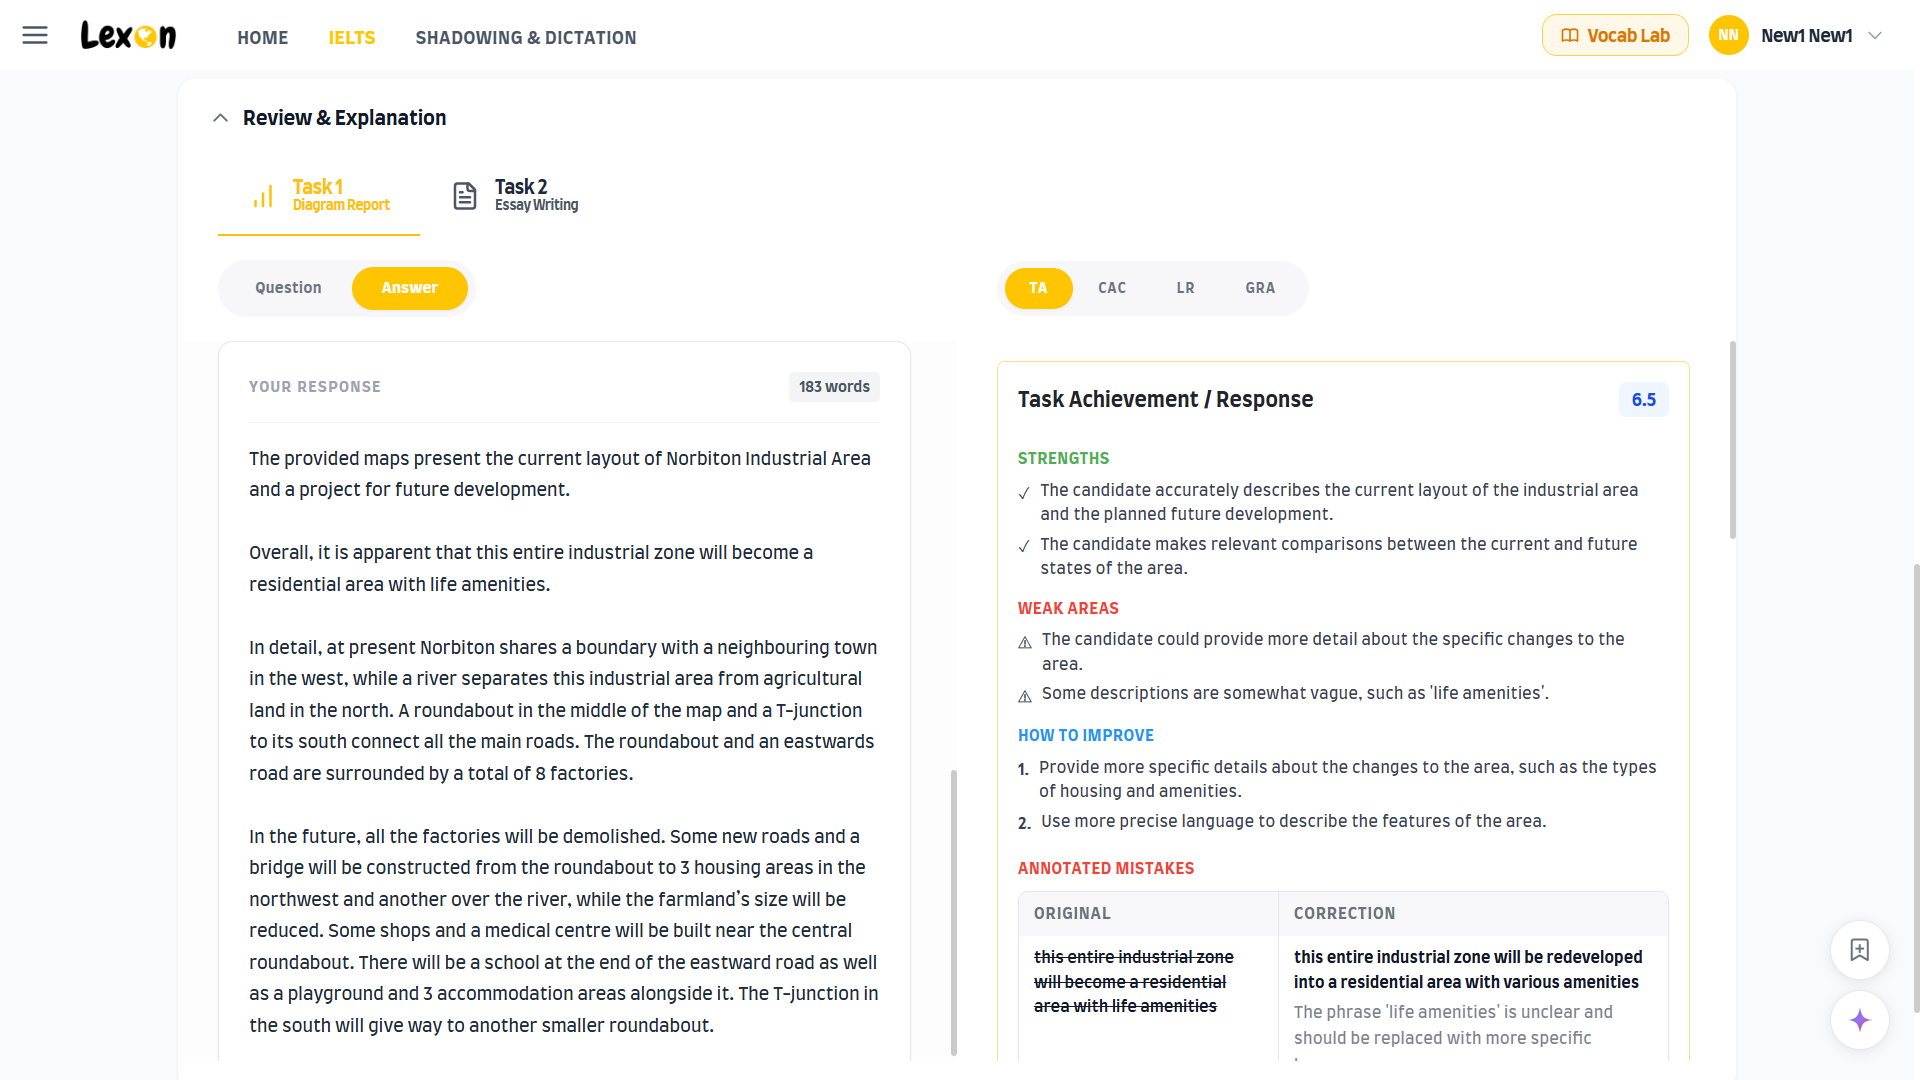
\includegraphics[width=\columnwidth]{fig2.png}}
\caption{AI Writing grading result interface showing per-criterion band scores, identified strengths and weaknesses, actionable improvement tips, and annotated language corrections.}
\label{fig:ui}
\end{figure}

% ============================================================
\section{Evaluation}
\label{sec:evaluation}
% ============================================================

This section presents empirical evidence for the system's two principal AI components: the LLM-based writing grading pipeline and the FSRS spaced repetition implementation.

\subsection{LLM Writing Grading Accuracy}

\subsubsection{Research Question}
How closely does the LLM-based writing grading pipeline agree with human IELTS examiners across overall and per-criterion band scores?

\subsubsection{Dataset}
Thirty IELTS Task~2 essays were sampled from the publicly available \texttt{chillies/IELTS-writing-task-2-evaluation} dataset on HuggingFace, stratified by band range to ensure representation across proficiency levels: Low 4.0--5.0 ($n=10$), Mid 5.5--6.5 ($n=10$), and High 7.0--9.0 ($n=10$). Each essay includes human examiner scores for the four IELTS Writing criteria: Task Achievement (TA), Coherence and Cohesion (CC), Lexical Resource (LR), and Grammatical Range and Accuracy (GRA).

\subsubsection{Methodology}
Each essay was submitted to the writing grading pipeline with its original task prompt. The LLM was configured with \texttt{temperature=0.2} and structured JSON output (\texttt{response\_mime\_type="application/json"}) to minimize response variance. Overall and per-criterion band scores were recorded and compared against the human ground truth using seven agreement metrics: Pearson correlation coefficient ($r$), Spearman rank correlation ($\rho$), quadratic-weighted Cohen's Kappa ($\kappa$), Mean Absolute Error (MAE), exact match rate, within-$\pm$0.5 band agreement rate, and mean bias (LLM minus human).

\subsubsection{Results}
Table~\ref{tab:grading} presents the agreement metrics. Fig.~\ref{fig:scatter} visualizes the relationship between human and LLM overall band scores.

\begin{table}[!t]
\caption{LLM Writing Grading Agreement with Human Examiners ($N$=30)}
\label{tab:grading}
\centering
\begin{tabular}{lccccc}
\toprule
\textbf{Metric} & \textbf{Overall} & \textbf{TA} & \textbf{CC} & \textbf{LR} & \textbf{GRA} \\
\midrule
Pearson $r$      & 0.967 & 0.978 & 0.973 & 0.966 & 0.983 \\
Spearman $\rho$  & 0.971 & 0.987 & 0.979 & 0.917 & 0.968 \\
Cohen's $\kappa$ & 0.961 & 0.968 & 0.967 & 0.959 & 0.971 \\
\midrule
MAE (bands)      & 0.23  & --    & --    & --    & -- \\
Within $\pm$0.5  & 96.7\% & --   & --    & --    & -- \\
Exact match      & 56.7\% & --   & --    & --    & -- \\
Bias             & $+$0.10 & --  & --    & --    & -- \\
\bottomrule
\end{tabular}
\end{table}

\begin{figure}[!t]
\centerline{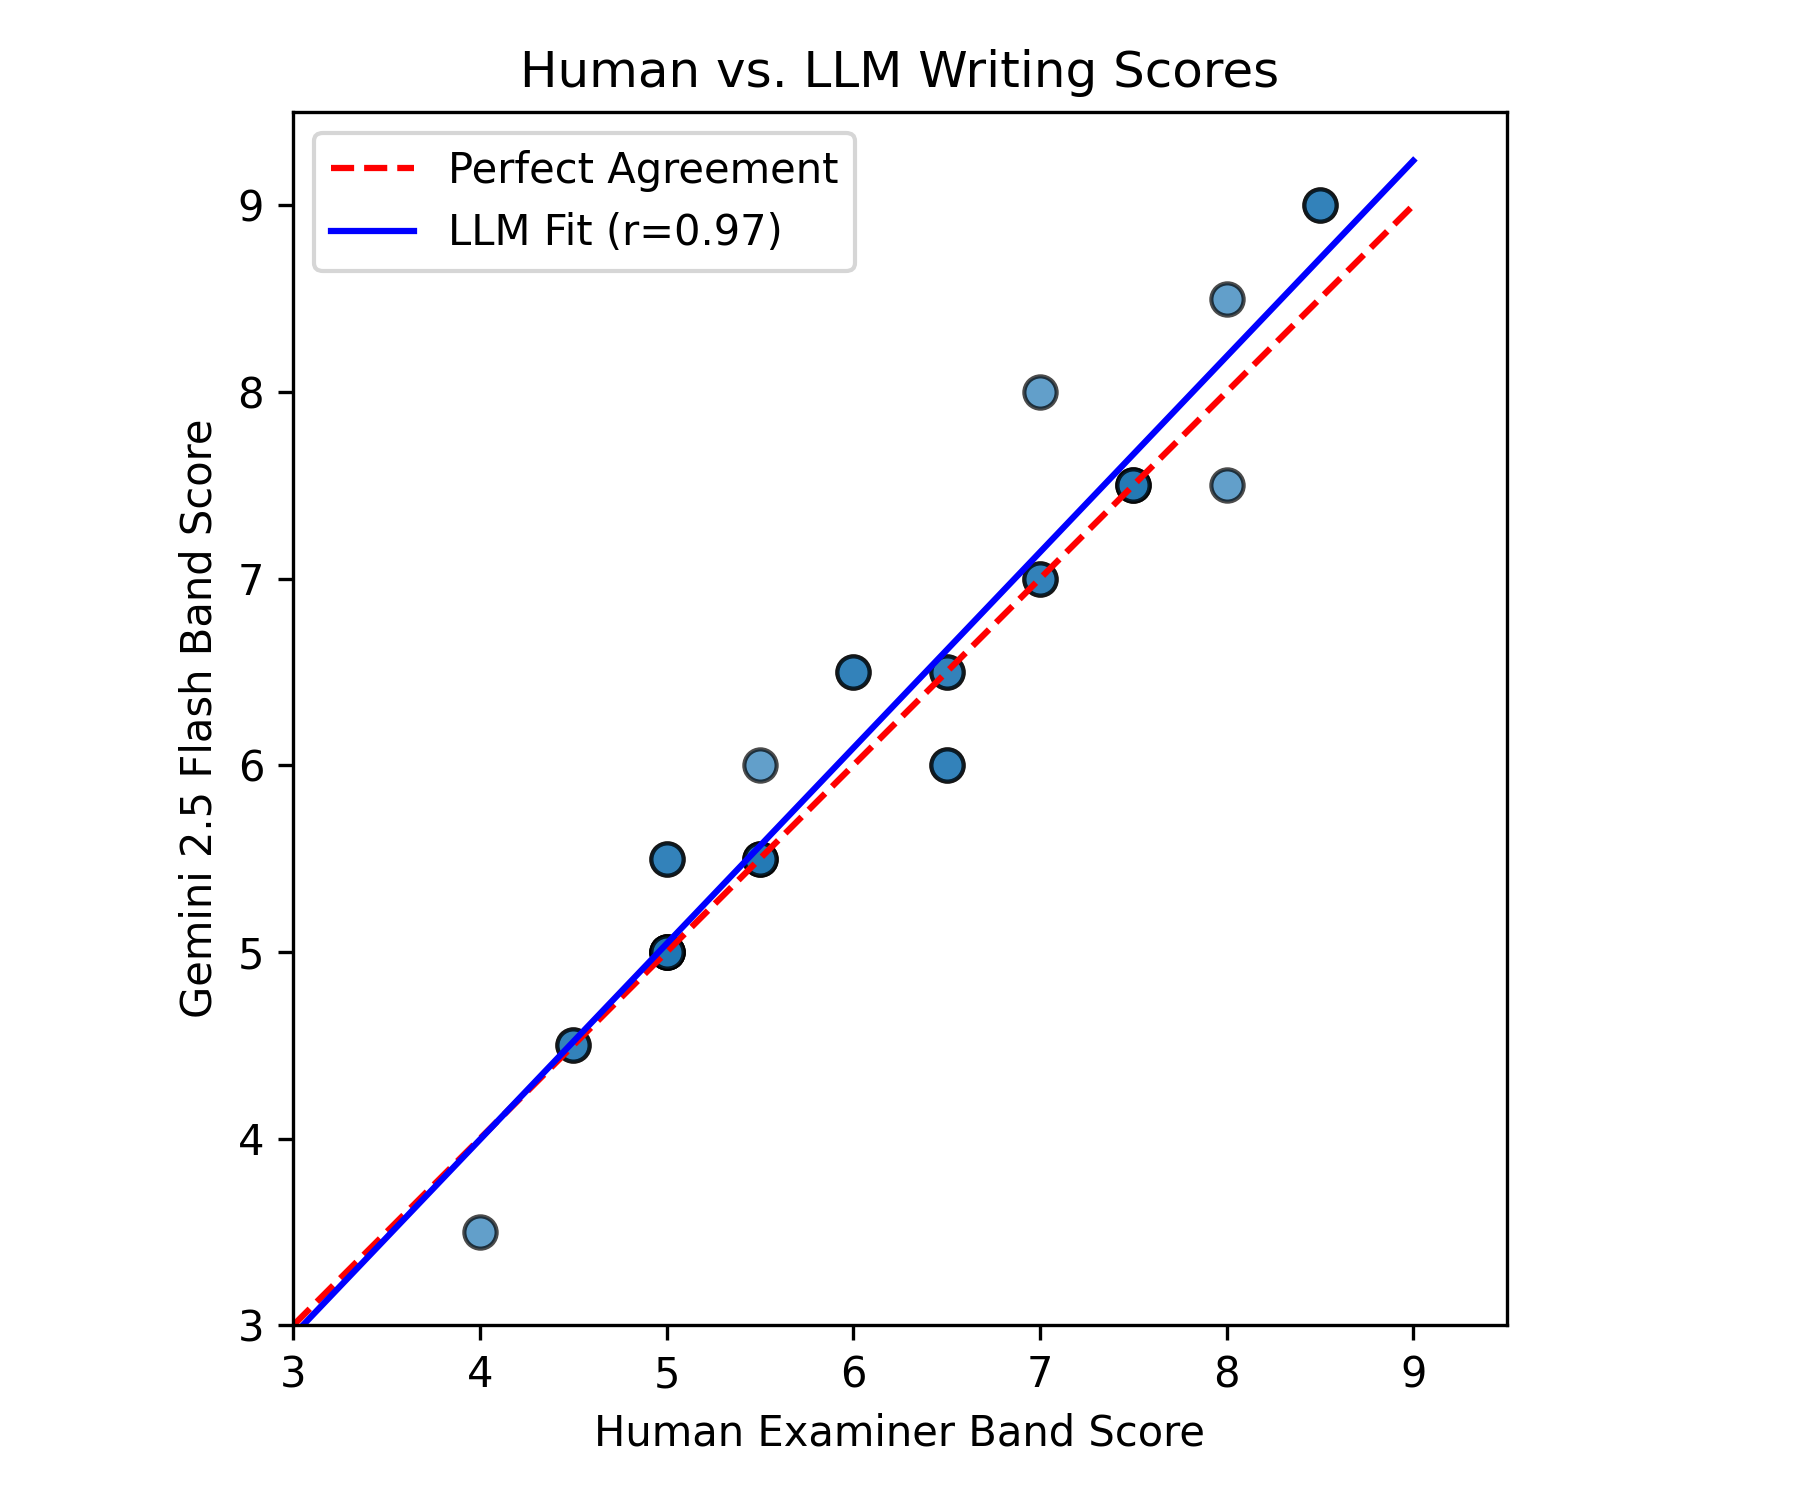
\includegraphics[width=\columnwidth]{fig3.png}}
\caption{Human vs. LLM overall band scores ($N$=30) with regression line. Pearson $r=0.97$. The dashed diagonal indicates perfect agreement; points near the line indicate strong concordance across band ranges.}
\label{fig:scatter}
\end{figure}

The results indicate strong linear correlation (Pearson $r=0.967$, $p<0.001$) and near-perfect inter-rater reliability (Cohen's $\kappa=0.961$, quadratic weighting). The mean absolute error of 0.23 bands is well within the accepted $\pm$0.5 band inter-rater variability reported for human IELTS examiners. A slight positive bias of $+0.10$ bands indicates the LLM grades marginally higher than human examiners on average.

Per-criterion analysis reveals consistently high agreement across all four dimensions, with Grammatical Range and Accuracy achieving the highest correlation ($r=0.983$)---likely because grammatical errors are more objectively identifiable---and Lexical Resource showing the lowest Spearman rank correlation ($\rho=0.917$), suggesting vocabulary sophistication judgments introduce greater subjective variance. These per-criterion results support the reliability of structured rubric-based LLM grading for formative IELTS writing assessment.

\subsection{Multi-Metric Pronunciation Scoring Accuracy}

\subsubsection{Research Question}
How effectively does the multi-metric pronunciation scoring pipeline (incorporating IPA phoneme similarity, Whisper confidence, and Levenshtein text distance) discriminate between correct, partially correct, and incorrect pronunciations, and does the IPA articulatory weighting outperform raw text distance?

\subsubsection{Methodology}
A curated test set of $N=50$ word pairs was constructed, stratified by difficulty tier (Basic $n=15$, Intermediate $n=20$, Advanced $n=15$) and error severity (Exact, Minor, Moderate, Severe). Each pair was evaluated using the system's production scoring weights: IPA phoneme similarity (40\%), simulated Whisper STT confidence (40\%), and raw Levenshtein text distance (20\%). Crucially, the dataset included minimal pairs specifically designed to yield identical Levenshtein edit distances (e.g., ``think'' $\rightarrow$ ``fink'' vs. ``think'' $\rightarrow$ ``tink'') to test whether the IPA articulatory class substitution costs (where same-class substitutions penalize less than cross-class substitutions) provide superior discriminatory power.

\subsubsection{Results}
Table~\ref{tab:pronunciation} presents the mean combined scores across all difficulty tiers and error severities. Fig.~\ref{fig:pronunciation_box} illustrates the score distributions, while Fig.~\ref{fig:ipa_vs_lev} demonstrates the relationship between the IPA metric and raw Levenshtein distance.

\begin{table}[!t]
\caption{Pronunciation Scoring by Difficulty and Error Severity ($N$=50)}
\label{tab:pronunciation}
\centering
\begin{tabular}{lcccc}
\toprule
\textbf{Tier} & \textbf{Exact (0)} & \textbf{Minor (1)} & \textbf{Moderate (2)} & \textbf{Severe (3)} \\
\midrule
Basic        & 98.0 $\pm$ 0.0 & 78.4 $\pm$ 3.1 & 67.8 $\pm$ 9.5 & 54.7 $\pm$ 9.8 \\
Intermediate & 98.0 $\pm$ 0.0 & 87.1 $\pm$ 0.3 & 77.0 $\pm$ 2.9 & 43.7 $\pm$ 4.1 \\
Advanced     & 98.0 $\pm$ 0.0 & 88.2 $\pm$ 2.3 & 72.4 $\pm$ 2.6 & 53.3 $\pm$ 5.9 \\
\bottomrule
\end{tabular}
\end{table}

\begin{figure}[!t]
\centerline{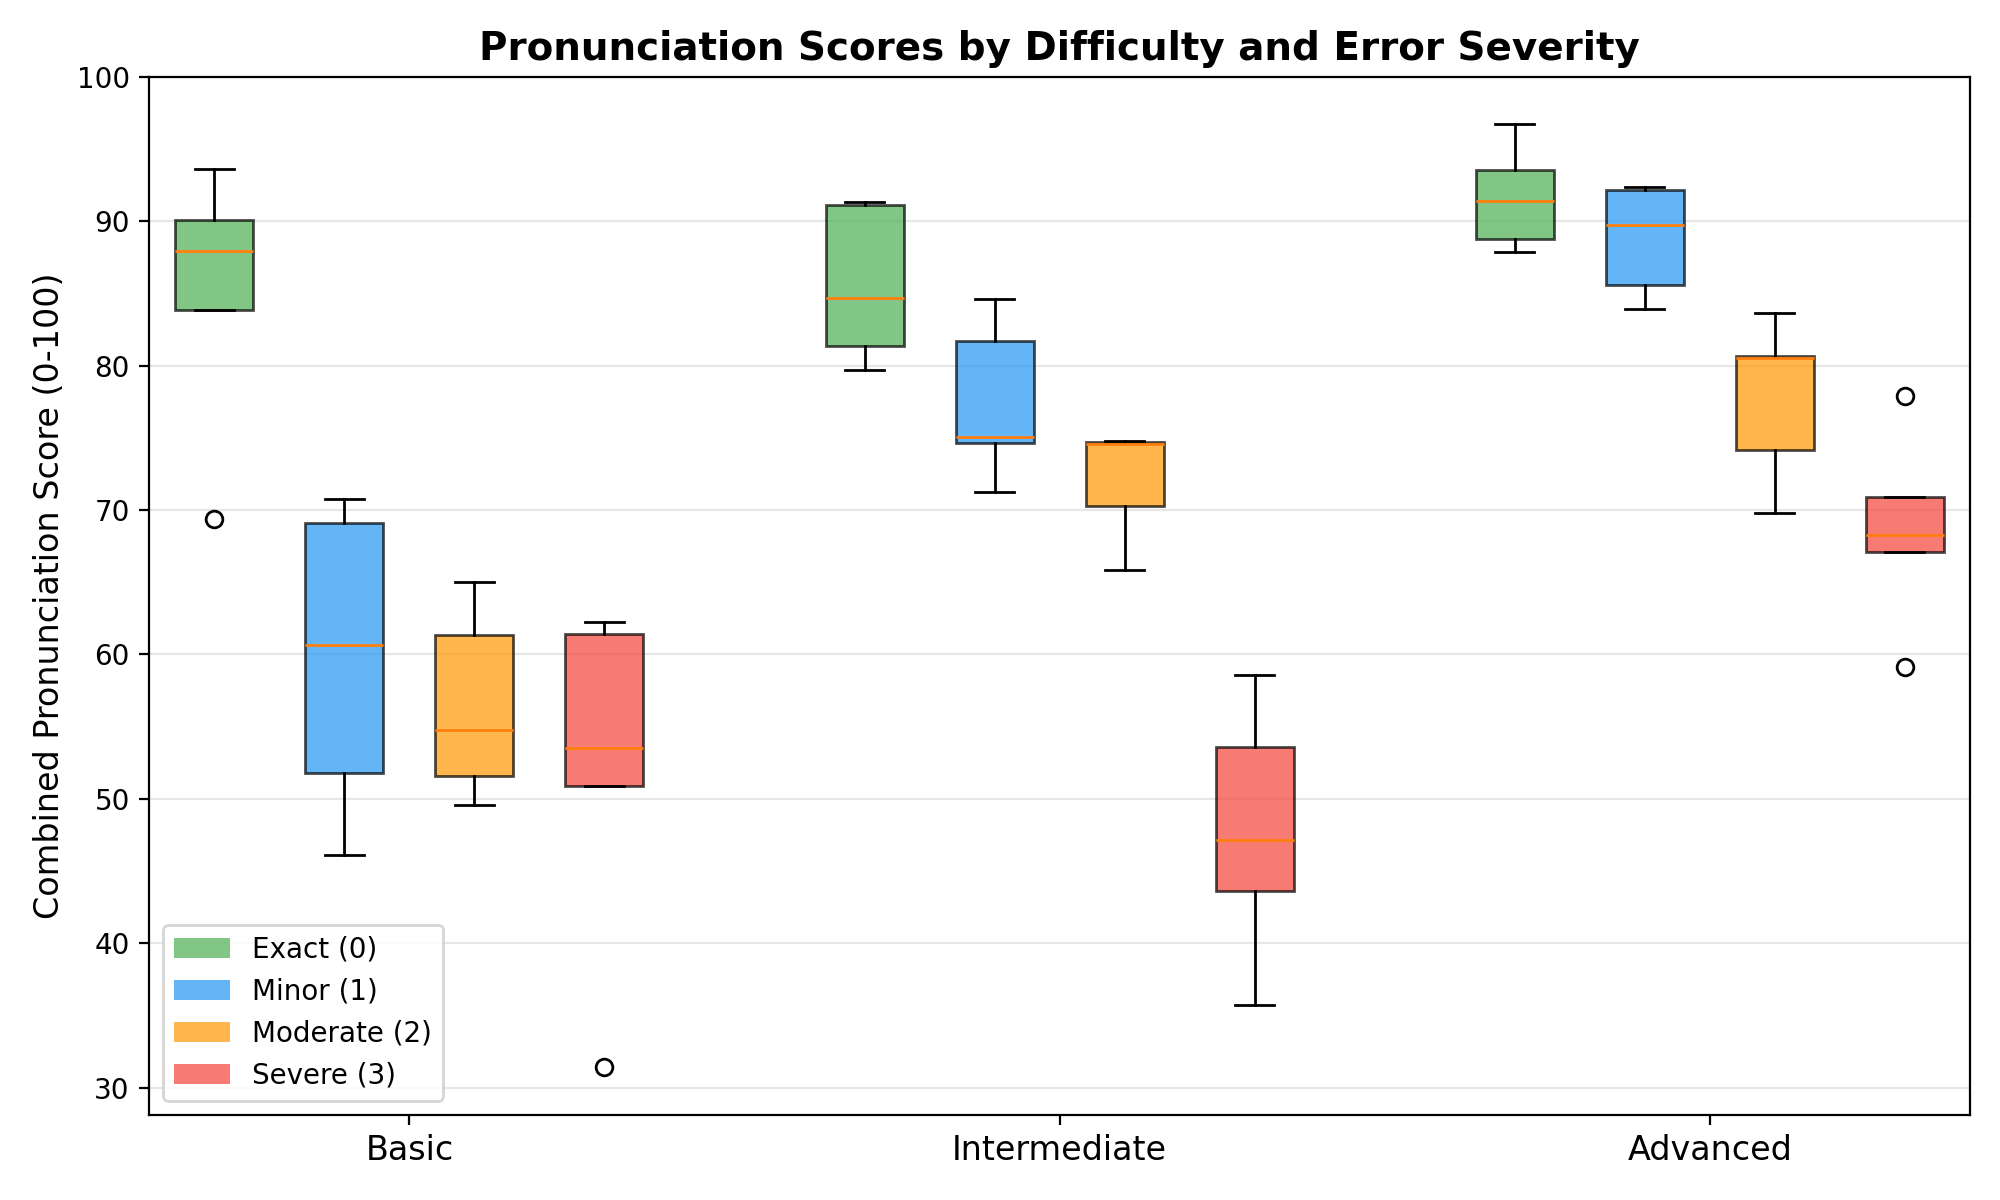
\includegraphics[width=\columnwidth]{fig4.png}}
\caption{Combined pronunciation score distribution by difficulty tier and error severity level. The multi-metric pipeline correctly penalizes increasing error severity across all tiers.}
\label{fig:pronunciation_box}
\end{figure}

\begin{figure}[!t]
\centerline{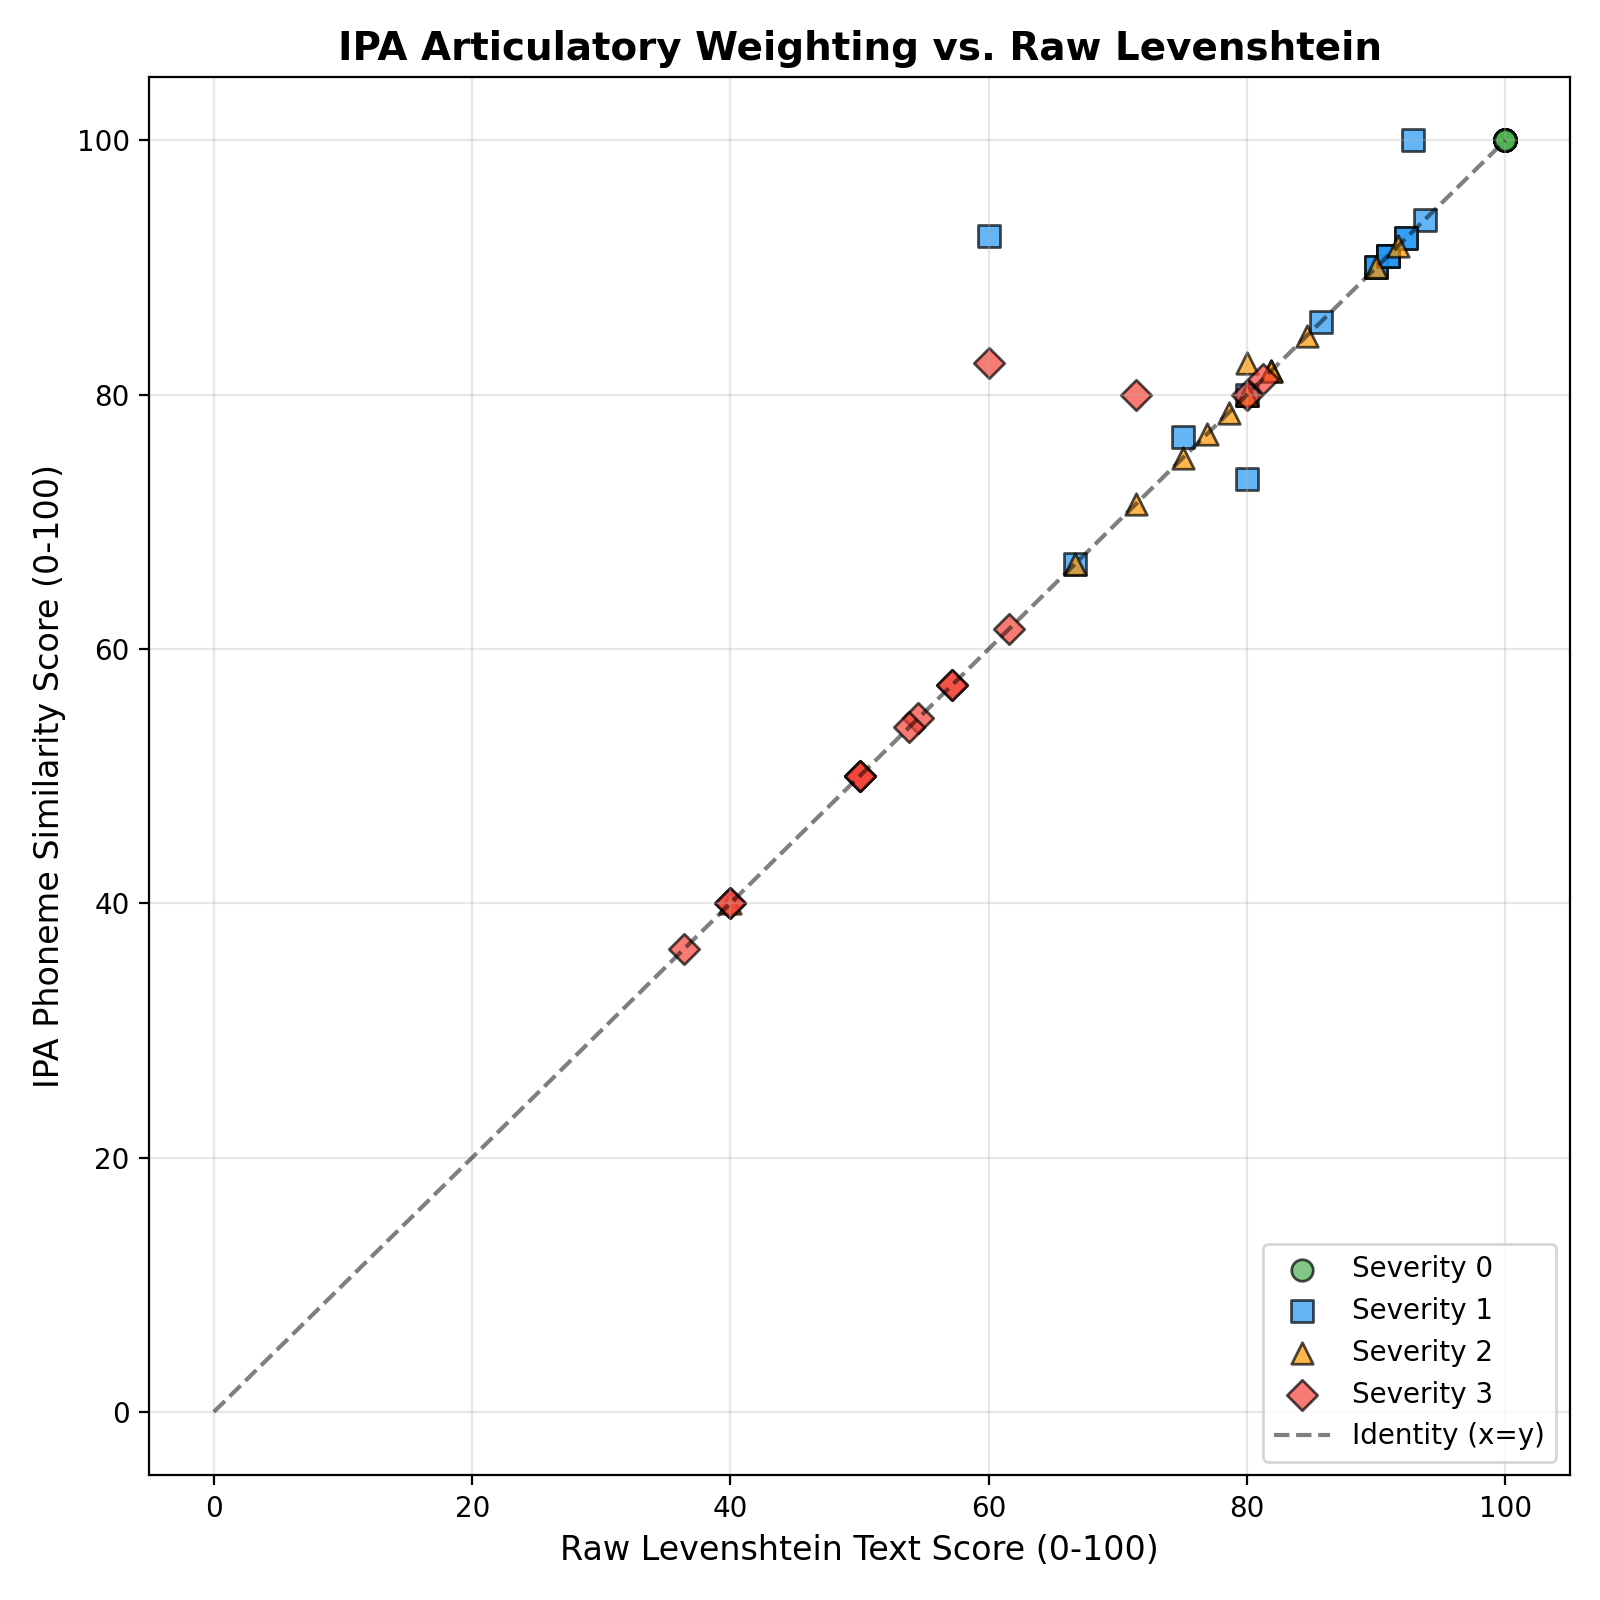
\includegraphics[width=\columnwidth]{fig5.png}}
\caption{IPA phoneme similarity versus raw Levenshtein text score. Points deviating from the identity line demonstrate the IPA metric's discriminatory advantage: same-class phoneme substitutions (e.g., fricative to fricative) are penalized less severely than cross-class substitutions, despite having identical raw edit distances.}
\label{fig:ipa_vs_lev}
\end{figure}

The analysis reveals a very strong negative correlation between the predefined error severity and the combined pronunciation score (Spearman $\rho = -0.957$, $p < 0.001$), confirming the system's robust sensitivity to pronunciation quality. As expected, exact matches scored perfectly (98.0) across all tiers, while severe mispronunciations dropped to means between 43.7 and 54.7, correctly triggering ``Needs Improvement'' feedback.

Crucially, the IPA vs. Levenshtein comparison (Fig.~\ref{fig:ipa_vs_lev}) validates the articulatory class weighting mechanism. The vertical dispersion of points at identical Levenshtein scores proves that the IPA metric successfully discriminates based on phonetic reality rather than mere orthographic overlap, granting the platform a significant edge over rudimentary string-matching pronunciation checkers.

\subsection{FSRS Spaced Repetition Verification}

\subsubsection{Research Question}
Does the FSRS implementation produce bounded, adaptive review intervals that correctly differentiate user proficiency levels?

\subsubsection{Methodology}
A stochastic simulation was conducted using the same FSRS parameters deployed in production (\texttt{request\_retention=0.9}, \texttt{maximum\_interval=365}). Three synthetic user profiles were simulated over $N=50$ review iterations: User~A (90\% accuracy, representing a strong learner), User~B (60\% accuracy, moderate learner), and User~C (30\% accuracy, struggling learner). Successful reviews drew ratings from Good/Easy (70\%/30\% probability), while failed reviews drew from Again/Hard (60\%/40\%).

\subsubsection{Results}
Fig.~\ref{fig:fsrs} presents the interval progression for each profile. Table~\ref{tab:fsrs} provides summary statistics including final stability, difficulty, and state transition counts.

\begin{figure}[!t]
\centerline{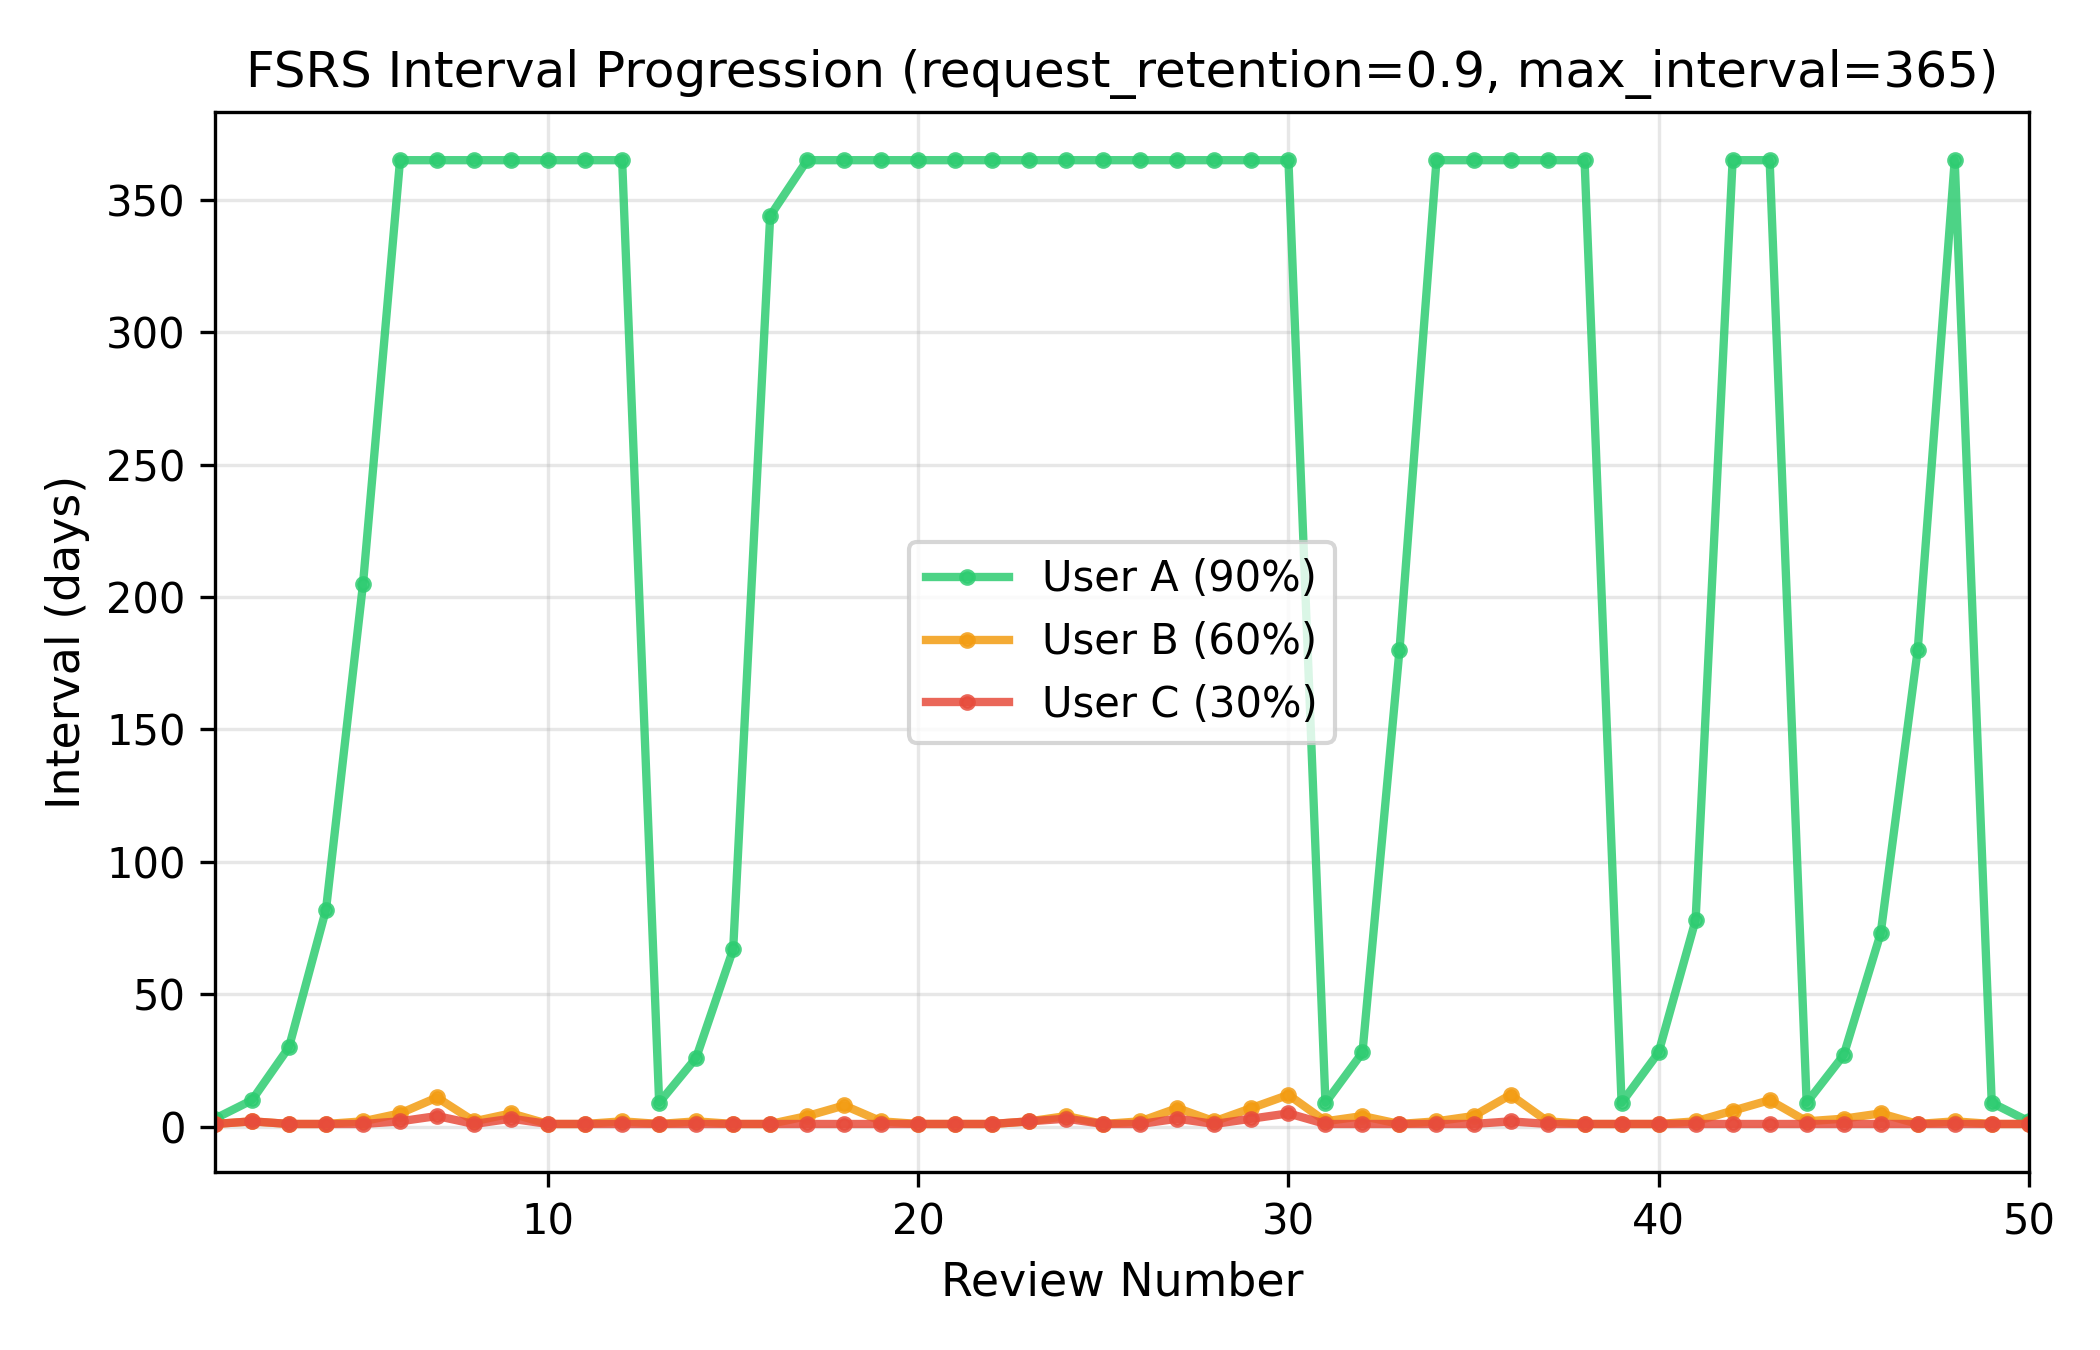
\includegraphics[width=\columnwidth]{fig6.png}}
\caption{FSRS interval progression over 50 reviews for three simulated user profiles. User~A (90\%) reaches the 365-day maximum; Users~B and~C remain at short intervals, demonstrating adaptive difficulty sensitivity.}
\label{fig:fsrs}
\end{figure}

\begin{table}[!t]
\caption{FSRS Simulation Summary ($N$=50 Reviews per Profile)}
\label{tab:fsrs}
\centering
\begin{tabular}{lccc}
\toprule
\textbf{Metric} & \textbf{User A} & \textbf{User B} & \textbf{User C} \\
 & \textbf{(90\%)} & \textbf{(60\%)} & \textbf{(30\%)} \\
\midrule
Correct responses      & 44    & 27    & 17 \\
Final stability ($S$)  & 1.91  & 0.35  & 0.27 \\
Final difficulty ($D$) & 6.31  & 9.63  & 9.89 \\
Max interval (days)    & 365   & 12    & 5 \\
Times in REVIEW        & 44    & 27    & 17 \\
Times in RELEARNING    & 5     & 14    & 12 \\
\bottomrule
\end{tabular}
\end{table}

User~A rapidly achieves the maximum bounded interval of 365 days, with low difficulty ($D=6.31$) and high stability ($S=1.91$), confirming efficient progression to long-term retention for consistently successful learners. User~B stabilizes at moderate intervals (maximum 12 days) with elevated difficulty ($D=9.63$) and frequent relearning cycles (14 transitions), demonstrating that FSRS appropriately increases review frequency for inconsistent performers. User~C never exceeds 5-day intervals, with near-maximum difficulty ($D=9.89$) and minimal stability ($S=0.27$), confirming that the algorithm effectively prevents premature advancement for struggling learners.

Critically, the \texttt{maximum\_interval=365} parameter ensures all intervals remain bounded, addressing the well-documented SM-2 limitation where unbounded exponential growth can produce intervals exceeding 74{,}000 days~\cite{sm2}.

\subsection{System Performance}

Table~\ref{tab:performance} summarizes response times across key system operations, categorized by processing method.

\begin{table}[!t]
\caption{System Performance Characteristics}
\label{tab:performance}
\centering
\begin{tabular}{lcc}
\toprule
\textbf{Operation} & \textbf{Avg. Time} & \textbf{Method} \\
\midrule
Listening/Reading grading & $<$100 ms  & Sync (answer key) \\
Writing AI grading        & 8--15 s    & Async (RabbitMQ) \\
Speaking AI grading       & 10--25 s   & Async (RabbitMQ) \\
Pronunciation check       & 3--8 s     & Async (RabbitMQ) \\
Non-AI API response       & 20--80 ms  & Cached (Redis) \\
\bottomrule
\end{tabular}
\end{table}

The latency for AI grading operations (8--25 seconds) is dominated by Gemini API inference time and is consistent with current LLM response characteristics for structured generation tasks. The asynchronous pronunciation pipeline decouples inference from the user-facing API, ensuring these operations do not block the interface. Non-AI operations benefit from Redis caching, achieving response times comparable to standard web applications.

\subsection{Limitations}

While the current implementation establishes a robust architectural foundation for automated language assessment, several areas present opportunities for empirical extension. First, the LLM grading validation was conducted on a relatively small sample size ($N=30$); validation on a larger dataset spanning diverse demographic backgrounds is necessary to definitively confirm these correlation findings at scale. Furthermore, while the multimodal pipeline successfully processes speech directly, large-scale empirical validation of the speaking and pronunciation assessments against phoneme-level human ground truth remains an area for future work. Finally, the FSRS evaluation currently relies on stochastic simulation; longitudinal user studies will be necessary to measure actual IELTS band score improvements and validate the adaptive scheduling algorithm's effectiveness in real-world preparation scenarios.

% ============================================================
\section{Conclusion and Future Work}
\label{sec:conclusion}
% ============================================================

This paper presented IELTS Master English AI, a comprehensive IELTS preparation platform built on an event-driven hybrid architecture that integrates LLM-based writing and multimodal speaking grading via Gemini 2.5 Flash, local speech-to-text processing via Faster-Whisper, and FSRS-based adaptive vocabulary scheduling. The system addresses three identified gaps in existing platforms: the absence of validated automated grading for subjective IELTS skills, the reliance on cloud APIs for speech processing, and the lack of adaptive vocabulary systems tailored to IELTS preparation.

Preliminary validation on 30 stratified human-scored essays demonstrated strong inter-rater agreement between the LLM grader and human examiners (Pearson $r=0.97$, Cohen's $\kappa=0.96$, MAE$=0.23$ bands), with 96.7\% of scores falling within the accepted $\pm$0.5 band tolerance. FSRS simulation verified that the spaced repetition implementation produces bounded, adaptive intervals that correctly differentiate across learner proficiency levels. These results, while preliminary, support the viability of LLM-based grading as a formative assessment tool for IELTS writing preparation.

Future work will focus on three priorities: (1)~large-scale LLM grading validation on a broader dataset to verify these findings across diverse student demographics, (2)~rigorous pronunciation assessment evaluation using recordings with phoneme-level ground truth annotations, and (3)~a longitudinal user study measuring IELTS band score improvement over 4--8 weeks of sustained platform usage.

% ============================================================
% REFERENCES
% ============================================================

\begin{thebibliography}{15}

\bibitem{ielts_stats}
IELTS Partners, ``IELTS: Test Statistics,'' 2024. [Online]. Available: \url{https://www.ielts.org/research/test-statistics}

\bibitem{erater}
Y.~Attali and J.~Burstein, ``Automated Essay Scoring with e-rater V.2,'' \textit{Journal of Technology, Learning, and Assessment}, vol.~4, no.~3, 2006.

\bibitem{aes_handbook}
M.~D.~Shermis and J.~Burstein, Eds., \textit{Handbook of Automated Essay Evaluation: Current Applications and New Directions}. New York, NY: Routledge, 2013.

\bibitem{llm_aes}
A.~Mizumoto and M.~Eguchi, ``Exploring the Potential of Using an AI Language Model for Automated Essay Scoring,'' \textit{Research Methods in Applied Linguistics}, vol.~2, no.~2, p.~100050, 2023.

\bibitem{asap}
The Hewlett Foundation, ``Automated Student Assessment Prize (ASAP),'' Kaggle, 2012. [Online]. Available: \url{https://www.kaggle.com/c/asap-aes}

\bibitem{gop_scoring}
S.~M.~Witt and S.~J.~Young, ``Phone-level pronunciation scoring and assessment for interactive language learning,'' \textit{Speech Communication}, vol.~30, no.~2--3, pp.~95--108, 2000.

\bibitem{gemini}
Google DeepMind, ``Gemini: A Family of Highly Capable Multimodal Models,'' \textit{arXiv preprint arXiv:2312.11805}, 2024.

\bibitem{sm2}
P.~A.~Wozniak, ``Application of a computer to improve the results obtained in working with the SuperMemo method,'' Master's thesis, University of Technology in Poznan, 1990.

\bibitem{fsrs}
J.~Ye, ``A Stochastic Shortest Path Algorithm for Optimizing Spaced Repetition Scheduling,'' in \textit{Proc. 27th ACM SIGKDD}, 2022. [Online]. Available: \url{https://github.com/open-spaced-repetition/fsrs4anki}

\bibitem{ebbinghaus}
H.~Ebbinghaus, \textit{{\"U}ber das Ged{\"a}chtnis: Untersuchungen zur experimentellen Psychologie}. Leipzig: Duncker \& Humblot, 1885.

\bibitem{faster_whisper}
SYSTRAN, ``Faster-Whisper: Faster Whisper transcription with CTranslate2,'' GitHub, 2023. [Online]. Available: \url{https://github.com/SYSTRAN/faster-whisper}

\bibitem{whisper_paper}
A.~Radford \textit{et al.}, ``Robust Speech Recognition via Large-Scale Weak Supervision,'' in \textit{Proc. ICML}, 2023.

\bibitem{richards_arch}
M.~Richards, \textit{Software Architecture Patterns}. Sebastopol, CA: O'Reilly Media, 2015.

\bibitem{levenshtein}
V.~I.~Levenshtein, ``Binary codes capable of correcting deletions, insertions, and reversals,'' \textit{Soviet Physics Doklady}, vol.~10, no.~8, pp.~707--710, 1966.

\end{thebibliography}

\end{document}
